\documentclass[border=10pt]{standalone}
\usepackage[svgnames]{xcolor}
\usepackage{amsmath}
\usepackage{pgfplots}
\pgfplotsset{compat=newest}
\usepackage[sfdefault]{FiraSans}
\usepackage{FiraMono}
\renewcommand*\familydefault{\sfdefault}
\begin{document}
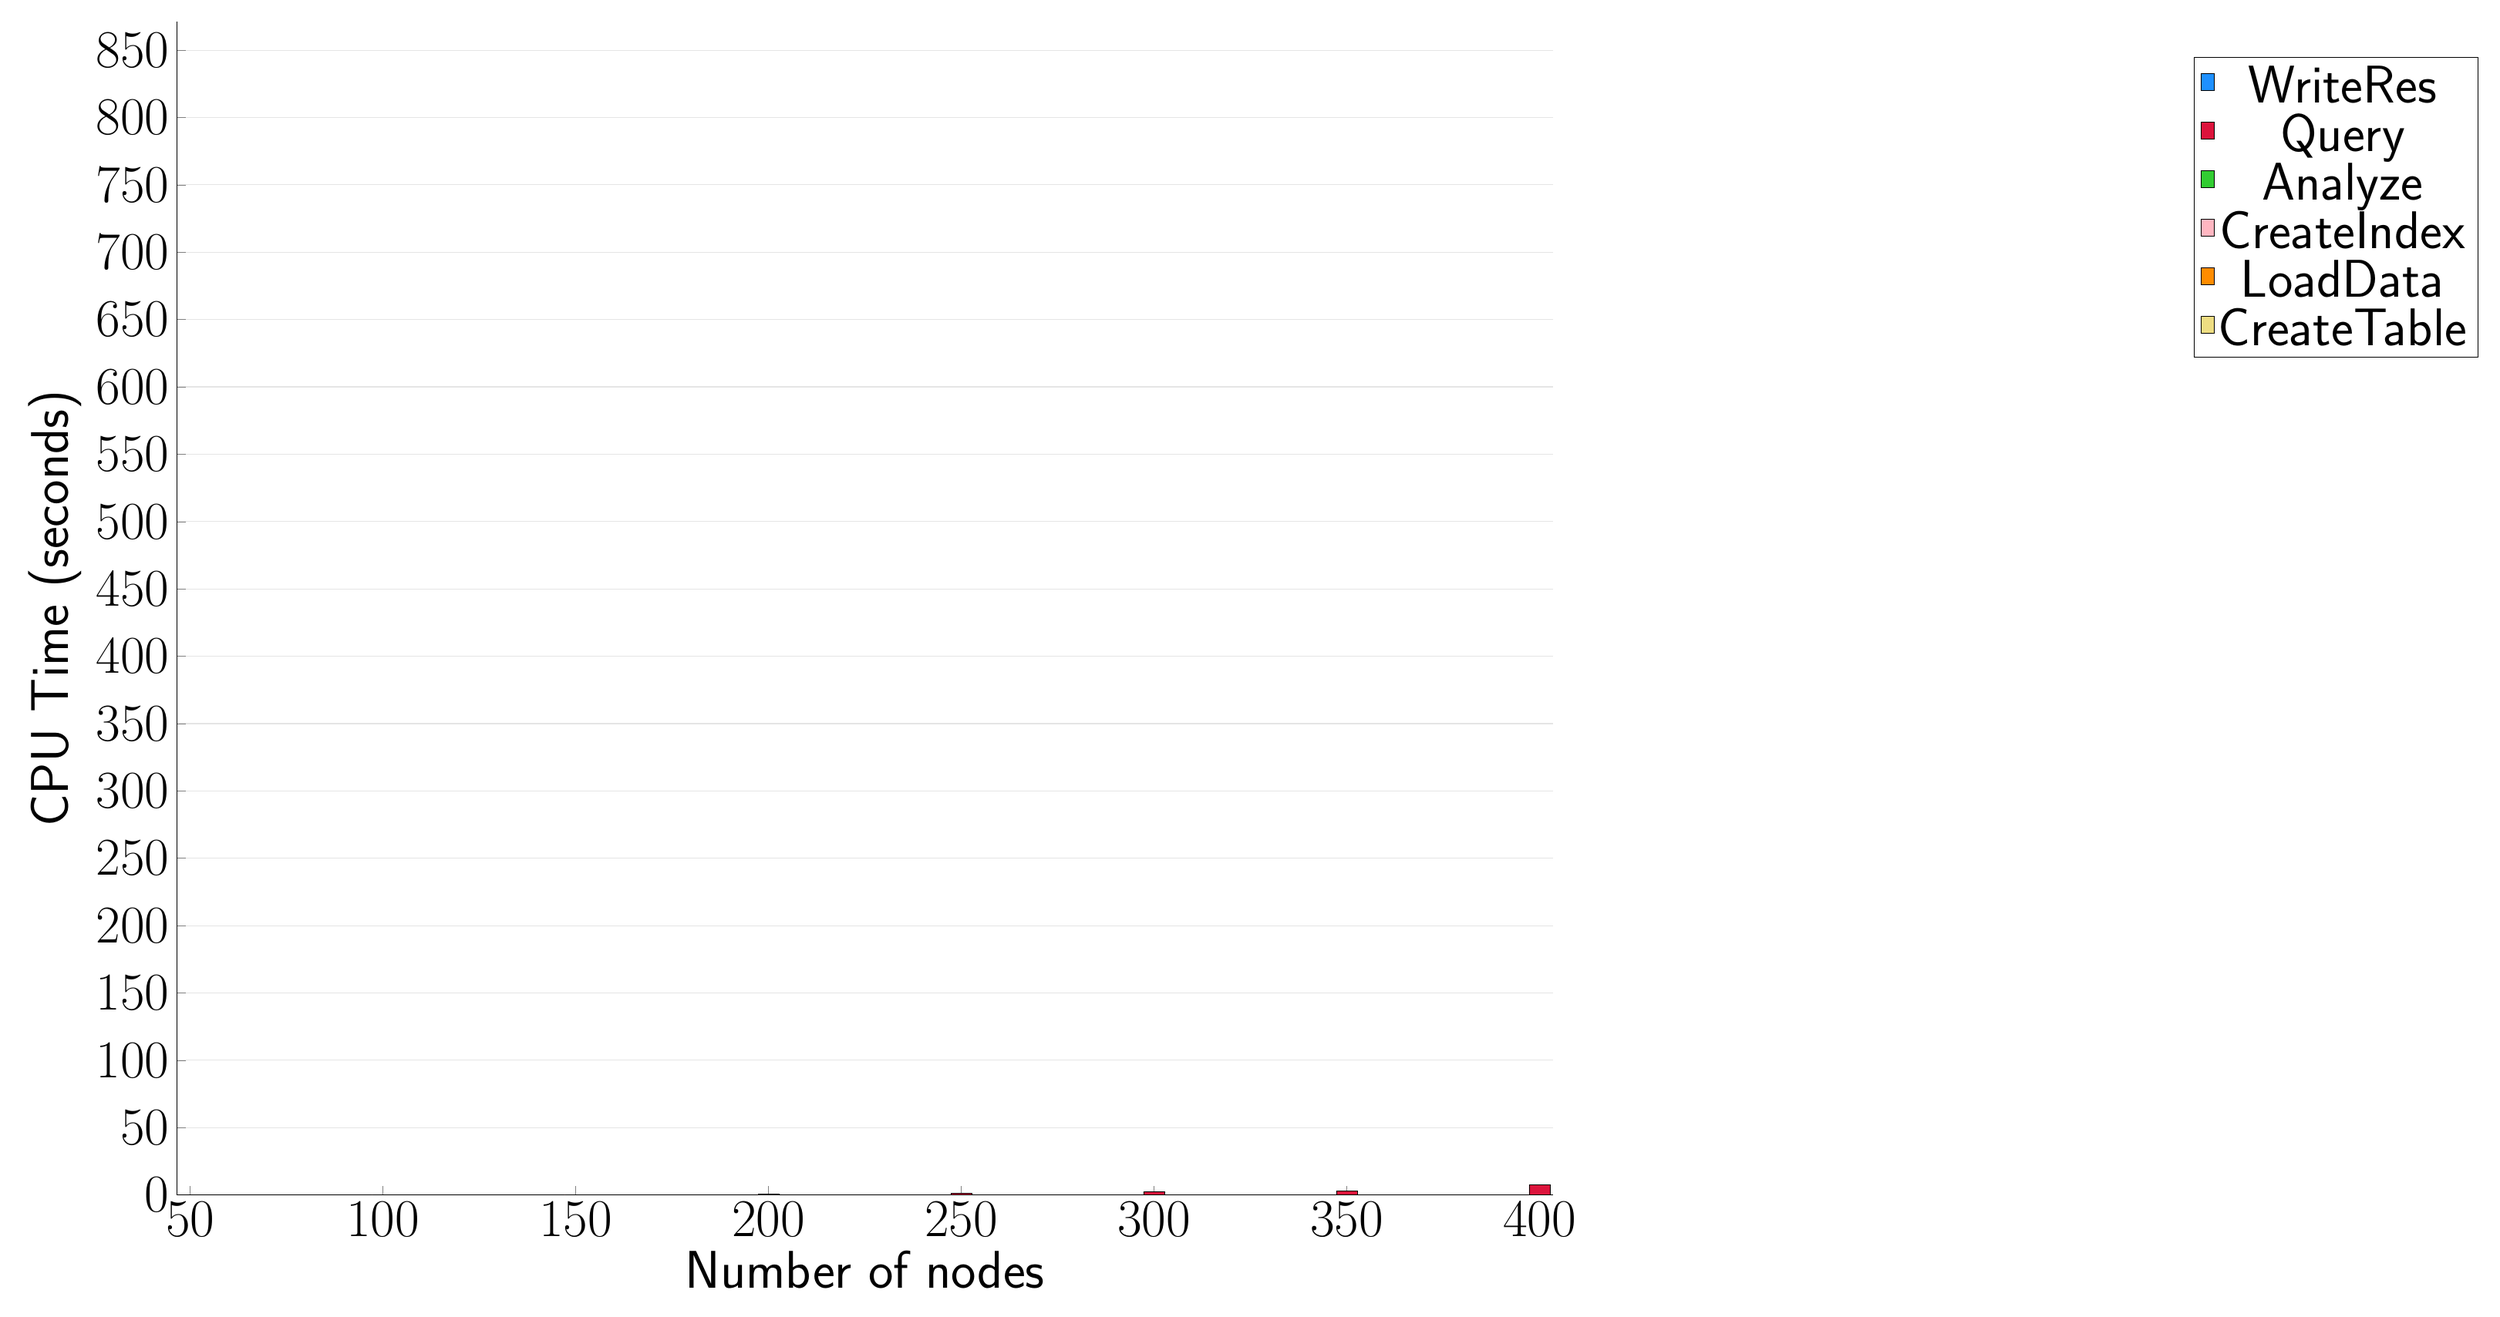
\begin{tikzpicture}
\begin{axis}[
   ybar stacked,
   width=2\textwidth,
   bar width=0.35cm,
   ymajorgrids, tick align=inside,
   major grid style={draw=gray!20},
   xtick=data,
   ymin=0, ymax=871.1066666692495,
   axis x line*=bottom,
   axis y line*=left,
   enlarge x limits=0.01,
   legend style={
       at={(1.6720000000000002, 0.97)},
       anchor=north east,
       legend columns=1,
       font=\Huge,
   },
   ylabel={CPU Time (seconds)},
   xlabel={Number of nodes},
   label style={font=\Huge},
   tick label style={font=\Huge},
]
\addlegendimage{fill=DodgerBlue, draw=black, line width=0.2pt}
\addlegendentry{WriteRes}
\addlegendimage{fill=Crimson, draw=black, line width=0.2pt}
\addlegendentry{Query}
\addlegendimage{fill=LimeGreen, draw=black, line width=0.2pt}
\addlegendentry{Analyze}
\addlegendimage{fill=LightPink, draw=black, line width=0.2pt}
\addlegendentry{CreateIndex}
\addlegendimage{fill=DarkOrange, draw=black, line width=0.2pt}
\addlegendentry{LoadData}
\addlegendimage{fill=LightGoldenrod, draw=black, line width=0.2pt}
\addlegendentry{CreateTable}
\addplot +[fill=LightGoldenrod, draw=black, line width=0.2pt] coordinates {
(50, 0.0)
(100, 0.003333333333333336)
(150, 0.006666666666666654)
(200, 0.006666666666666651)
(250, 0.003333333333333318)
(300, 0.003333333333333332)
(350, 0.003333333333333336)
(400, 0.003333333333333318)
};
\addplot +[fill=DarkOrange, draw=black, line width=0.2pt] coordinates {
(50, 0.003333333333333318)
(100, 0.0066666666666666706)
(150, 0.009999999999999988)
(200, 0.013333333333333343)
(250, 0.030000000000000002)
(300, 0.023333333333333334)
(350, 0.026666666666666682)
(400, 0.04666666666666667)
};
\addplot +[fill=LightPink, draw=black, line width=0.2pt] coordinates {
(50, 0.006666666666666672)
(100, 0.00999999999999999)
(150, 0.013333333333333324)
(200, 0.013333333333333343)
(250, 0.02000000000000002)
(300, 0.03666666666666668)
(350, 0.03999999999999998)
(400, 0.06)
};
\addplot +[fill=LimeGreen, draw=black, line width=0.2pt] coordinates {
(50, 0.0)
(100, 0.0)
(150, 0.0)
(200, 0.0)
(250, 0.0)
(300, 0.0)
(350, 0.003333333333333336)
(400, 0.0)
};
\addplot +[fill=Crimson, draw=black, line width=0.2pt] coordinates {
(50, 0.016666666666666677)
(100, 0.07666666666666667)
(150, 0.27666666666666667)
(200, 0.58)
(250, 1.3833333333333335)
(300, 2.3266666666666667)
(350, 2.9233333333333333)
(400, 7.273333333333333)
};
\addplot +[fill=DodgerBlue, draw=black, line width=0.2pt] coordinates {
(50, 0.0)
(100, 0.003333333333333336)
(150, 0.006666666666666672)
(200, 0.003333333333333336)
(250, 0.016666666666666673)
(300, 0.013333333333333345)
(350, 0.013333333333333272)
(400, 0.036666666666666924)
};
\end{axis}
\end{tikzpicture}

\end{document}
